\documentclass[xcolor={dvipsnames}]{beamer}
\usetheme{default}
\usepackage{amsmath, amssymb, upgreek, textcomp}
\usepackage{graphicx, float, subcaption}
\usepackage{hyperref}
\usepackage[numbered]{mcode}
\graphicspath{{Figures/}}

\makeatletter
\newcommand{\Spvek}[2][r]{%
	\gdef\@VORNE{1}
	\left[\hskip-\arraycolsep%
	\begin{array}{#1}\vekSp@lten{#2}\end{array}%
	\hskip-\arraycolsep\right]}

\def\vekSp@lten#1{\xvekSp@lten#1;vekL@stLine;}
\def\vekL@stLine{vekL@stLine}
\def\xvekSp@lten#1;{\def\temp{#1}%
	\ifx\temp\vekL@stLine
	\else
	\ifnum\@VORNE=1\gdef\@VORNE{0}
	\else\@arraycr\fi%
	#1%
	\expandafter\xvekSp@lten
	\fi}
\makeatother
\newcommand{\trans}{\text{T}}


\title{Introduction to Spectral Methods}
\subtitle{Numerical Solution of Poisson's Equation}


\author{Pablo Brubeck\inst{}}
\institute[ITESM]{
	\inst{}
	Department of Physics\\
	Tecnologico de Monterrey
}

\titlegraphic{
	
\includegraphics[width=3cm]{SPIELogo}
}

\date{October 7, 2016}
\subject{Numerical Analysis}

\AtBeginSection[]{
	\begin{frame}<beamer>{Outline}
		\tableofcontents[currentsection]
	\end{frame}
}

\begin{document}

\begin{frame}
	\titlepage
\end{frame}

\begin{frame}{Outline}
	\tableofcontents
	% You might wish to add the option [pausesections]
\end{frame}


\section{Poisson's Equation}
\begin{frame}{Poisson's Equation}{}

We are interested to find the function $u(x,y,z)$ that satisfies the boundary value problem

\begin{equation*}
\nabla^2 u = f
\end{equation*}

Subject to boundary conditions $u(C)=g$.

\pause
\bigskip
Where the laplacian operator is $\nabla^2=\frac{\partial^2}{\partial x^2}+\frac{\partial^2}{\partial y^2}+\frac{\partial^2}{\partial z^2}$.

\pause
\bigskip
When $f=0$, we have Laplace's equation as a special case.
\end{frame}


\begin{frame}{Poisson's Equation has many important applications.}{}
\begin{itemize}[<+->]
\item Electrostatics $\nabla^2 V = - \rho/\upvarepsilon_0$
\item Newtonian gravity $\nabla^2 \phi = 4\pi G\rho$
\item Thermal equilibrium $\nabla^2 T = 0$
\item Incompressible fluid flow $\nabla^2 v = 0, \nabla^2 p = f(\nu,V)$
\item Mechanical Engineering 
\item Image processing
\item And much more ...
\end{itemize}

\end{frame}


\section{One dimension}
\begin{frame}{Poisson's Equation in one dimension}{}
\begin{equation*}
\frac{d^2u}{dx^2}=f(x)
\end{equation*}
\vfill
Subject to $u(a)=g_1$ and  $u(b)=g_2$.

\bigskip
It is not always possible to integrate twice to find the solution.
\end{frame}

\begin{frame}{We must translate this continuous problem\\into a discrete one.}{}
	
For the space coordinate $x\in[a,b]$, we choose $n$ nodes $\left\{x_i\right\}_{i=1}^n$ on which we would like to know the value of $u(x_i)=u_i$.

\bigskip
Input $u_1$, $u_n$, $\vec{x}=\Spvek[c]{x_1;x_2;\vdots;x_n}$, and $\vec{f}=\Spvek[c]{f(x_1);f(x_2);\vdots;f(x_n)}$; output $\vec{u}=\Spvek[c]{u_1;u_2;\vdots;u_n}$.
\end{frame}

\begin{frame}{The discrete solution must solve the continuous problem.}{}
Is there a way to express $u(x)$ in terms of $u_i$?
\begin{equation*}
u(x) = \sum_j u_j \delta_j(x)
\end{equation*}

\pause
We introduce the cardinal functions $\delta_j(x)$.
\begin{equation*}
u(x_i) = \sum_j u_j \delta_j(x_i) = u_i
\end{equation*}

\pause
\begin{equation*}
\delta_j(x_i)=\begin{cases}
1, & i=j\\
0, & i\neq j
\end{cases}
\end{equation*}
\end{frame}

\begin{frame}{This is how the cardinal functions look like.}{}
\begin{figure}
\centering
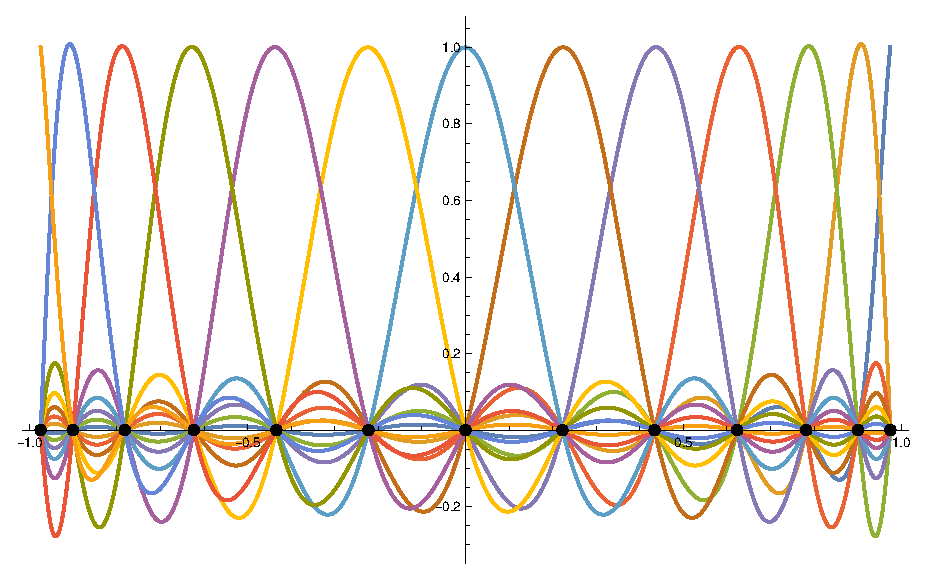
\includegraphics[width=\linewidth]{CardinalChebyshev}
\label{fig:CardinalChebyshev}
\end{figure}

\end{frame}
	

\begin{frame}{Now differentiate the expansion in cardinal functions.}{}
	
\begin{equation*}
u'(x_i)= \sum_j u_j \delta'_j(x_i)
\end{equation*}

\pause
We have found a matrix $D_{ij}=\delta'_j(x_i)$ that operates as a derivative.
\begin{equation*}
\frac{d}{dx}\vec{u} = D \vec{u}
\end{equation*}

\pause
\begin{equation*}
\frac{d^2}{dx^2}\vec{u} = D^2 \vec{u} = \vec{f}
\end{equation*}
\end{frame}

\begin{frame}{Solve the system of linear equations.}{}
\begin{equation*}
D^2 \vec{u} = \vec{f}
\end{equation*}
\pause
Recall that $\color{red} u_1$ and $\color{blue} u_n$ were given as boundary conditions.
\pause
\begin{equation*}
\begin{bmatrix}
\color{red} D^2_{11} & \color{ForestGreen} D^2_{1j} & \color{blue} D^2_{1n} \\
\color{red} D^2_{i1} & \color{ForestGreen} D^2_{ij} & \color{blue} D^2_{in} \\
\color{red} D^2_{n1} & \color{ForestGreen} D^2_{nj} & \color{blue} D^2_{nn}
\end{bmatrix}
\Spvek[c]{\color{red} u_1; \color{ForestGreen} u_j; \color{blue} u_n}=
{\color{red} \Spvek[c]{D^2_{11}; D^2_{i1}; D^2_{n1}}u_1}
+{\color{ForestGreen} \Spvek[c]{D^2_{1j}; D^2_{ij}; D^2_{nj}}\Spvek[c]{u_j}}
+{\color{blue} \Spvek[c]{D^2_{1n}; D^2_{in}; D^2_{nn}}u_n}
=\Spvek[c]{f_1; f_i; f_n}
\end{equation*}
With $i$ and $j$ ranging from 2 to $n-1$.

\bigskip
We have $n-2$ unknowns, but still $n$ equations.
\end{frame}

\begin{frame}{Discard the first and last rows.}{}
$\nabla^2u=f$ will not hold true at the boundary, but we will ensure the boundary conditions.
\begin{align*}
\color{ForestGreen} \Spvek[c]{D^2_{ij}}\Spvek[c]{u_j}&=
\Spvek[c]{f_i}
-{\color{red} u_1\Spvek[c]{D^2_{i1}}}
-{\color{blue} u_n\Spvek[c]{D^2_{in}}}\\
\color{ForestGreen}\Spvek[c]{u_j}&={\color{ForestGreen}\Spvek[c]{D^2_{ij}}^{-1}}
\Spvek[c]{f_i-{\color{red}u_1D^2_{i1}}-{\color{blue}u_nD^2_{in}}}
\end{align*}
With $i$ and $j$ ranging from 2 to $n-1$.
\end{frame}

\begin{frame}{Cardinal functions are obtained\\from a mother function.}{}
Usually we chose an orthogonal polynomial. It all depends on the domain of your solution.

\bigskip
\begin{tabular}{lll}
Chebysheb & $\Psi_n(x) = T_n(x)$ & $x\in[-1,1]$\\
Legendre  & $\Psi_n(x) = P_n(x)$ & $x\in[-1,1]$\\
Hermite   & $\Psi_n(x) = H_n(x)e^{-x^2/2}$ & $x\in(-\infty,\infty)$\\
Laguerre  & $\Psi_n(x) = xL_{n-1}^{(1)}(x)e^{-x/2}$ & $x\in[0,\infty)$\\
\end{tabular}
\end{frame}

\begin{frame}{Cardinal functions are obtained\\from a mother function.}{}
Let $\Psi_n(x)$ be a function with $n$ roots on $\left\{x_i\right\}_{i=1}^n$, i. e. $\Psi_n(x_i)=0$.  By expanding $\Psi_n(x)$ around its roots we can find a expression for $\delta_j(x)$.
\pause
\begin{equation*}
\Psi_n(x)=0+\Psi'_n(x_j)(x-x_j)+\frac{\Psi''_n(x_j)}{2}(x-x_j)^2+O((x-x_j)^3)
\end{equation*}
\pause
\begin{equation*}
\delta_j(x)=\frac{\Psi_n(x)}{(x-x_j)\Psi'_n(x_j)}=1+\frac{\Psi''_n(x_j)}{2\Psi'_n(x_j)}(x-x_j)+O((x-x_j)^2)
\end{equation*}
\end{frame}


\begin{frame}{Differentiate to obtain the elements of $D$.}{}
\begin{equation*}
D_{ij}=\delta'_j(x_i)=\frac{1}{x_i-x_j}\frac{\Psi'_n(x_i)}{\Psi'_n(x_j)}, \qquad i\neq j
\end{equation*}

\bigskip
The diagonal is a bit tricky.
\begin{equation*}
D_{jj}=\delta'_j(x_j)=\frac{\Psi_n''(x_j)}{2\Psi_n'(x_j)}
\end{equation*}
\end{frame}

\begin{frame}[fragile]{MATLAB code}{}
Solve Poisson's equation
\begin{equation*}
\frac{d^2u}{dx^2}=1000\cos(5\pi x)e^{-x^2}
\end{equation*}

with boundary conditions $u(-1)=2$, $u(1)=-1$.
\pause
\begin{lstlisting}
[D,x]=chebD(n); D2=D*D;   % Differentiation matrix and nodes
f=1000*cos(5*pi*x).*exp(-x.^2); % Source term
u=zeros(n,1); u([1,n])=[-1,2];  % Impose boundary conditions
% Solve and plot
u(2:n-1)=D2(2:n-1,2:n-1)\(f(2:n-1)-D2(2:n-1,[1,n])*u([1,n]));
plot(x,u);
\end{lstlisting}
\end{frame}

\begin{frame}{Here is our solution.}{}
\begin{figure}
\centering
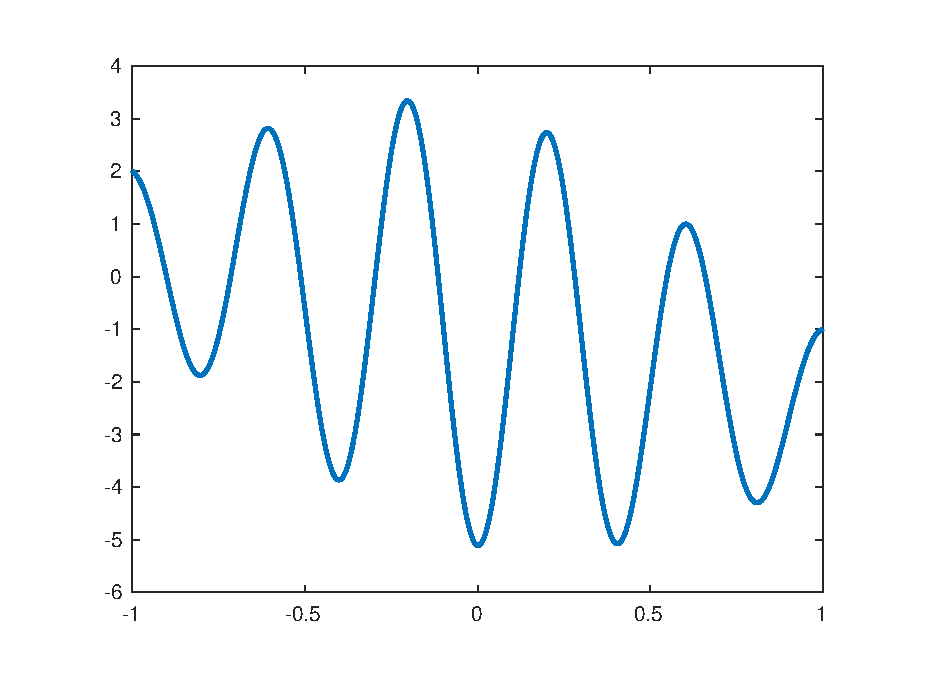
\includegraphics[width=\linewidth]{Figures/Poisson1D}
\label{fig:Poisson1D}
\end{figure}
\end{frame}




\section{Two Dimensions}

\begin{frame}{Poisson's Equation in two dimensions}{}
Our domain of solution will be the rectangle $[a,b] \times [c,d]$
\begin{equation*}
\frac{\partial^2 u}{\partial x^2}+\frac{\partial^2 u}{\partial y^2}=f(x,y)
\end{equation*}
Subject to boundary conditions 
\begin{equation*}
u(x,y)=\begin{cases}
g_1(y), & x=a\\
g_2(y), & x=b\\
h_1(x), & y=c\\
h_2(x), & y=d
\end{cases}
\end{equation*}

\end{frame}

\begin{frame}{In 2D we use matrices for $u$ and $f$.}{}

\begin{align*}
u(x_i, y_j) &= u_{ij}\\
f(x_i, y_j) &= f_{ij}
\end{align*}

\begin{equation*}
u(x,y)=\sum_{k,l}u_{kl}\delta_k(x)\delta_l(y)
\end{equation*}

\end{frame}

\begin{frame}{Multiplying times $D$ does the job of partial derivatives.}{}
\begin{equation*}
\frac{\partial u}{\partial x} = DU = \begin{bmatrix}
Du_{i1} & Du_{ij} & Du_{in}
\end{bmatrix}
\end{equation*}

\pause
\begin{equation*}
\frac{\partial u}{\partial y} = UD^\trans = (DU^\trans)^\trans = \begin{bmatrix}
(Du_{1i})^\trans \\ (Du_{ji})^\trans \\ (Du_{ni})^\trans
\end{bmatrix}
\end{equation*}

\pause
\begin{equation*}
\nabla^2 u = D^2 U + U (D^2)^\trans
\end{equation*}
\end{frame}

\begin{frame}{Now solve the system of linear equations.}{}
\begin{equation*}
D^2 U + U (D^2)^\trans = F
\end{equation*}
Boundary conditions are the tricky part.
\begin{equation*}
U={\color{red}\tilde{U}}+{\color{blue}U_B}=
{\color{red}\begin{bmatrix}
0 & 0 & 0\\
0 & u_{ij} & 0\\
0 & 0 & 0
\end{bmatrix}}+
{\color{blue}\begin{bmatrix}
u_{11} & u_{1j} & u_{1n}\\
u_{i1} &    0   & u_{in}\\
u_{n1} & u_{nj} & u_{nn}\\
\end{bmatrix}}
\end{equation*}
\begin{equation*}
D^2{\color{red}\tilde{U}} + {\color{red}\tilde{U}}(D^2)^\trans = F - D^2 {\color{blue}U_B} - {\color{blue}U_B} (D^2)^\trans = \tilde{F}
\end{equation*}
\end{frame}

\begin{frame}{Discard first and last rows and columns.}{}
$\nabla^2u=f$ will not hold true at the boundary, but we will ensure the boundary conditions.
\begin{equation*}
(D^2_{ij}) \tilde{U}_{ij} + \tilde{U}_{ij} (D^2_{ij})^\trans = \tilde{F}_{ij}
\end{equation*}
With $i$ and $j$ ranging from 2 to $n-1$.

\bigskip
Now we just have to solve $(n-2)^2 \times (n-2)^2$ system of linear equations.
\end{frame}

\begin{frame}{Matrix inversion does not help.}{}
A matrix equation of the form $AX+XB=C$ is known as a Sylvester equation.

\bigskip
There's a built-in MATLAB function that solves them.

\bigskip
\mcode{X=sylvester(A,B,C)}

\bigskip
This algorithm uses the Schur decomposition to solve a block-triangular matrix very efficiently. 
\end{frame}

\begin{frame}{Two dimensional example}{}
Solve Laplace's equation on $(x,y)\in[-1,1]\times[-1,1]$
\begin{equation*}
\nabla^2 u=0
\end{equation*}

with boundary conditions 
\begin{equation*}
u(x,y)=\begin{cases}
\sin^4(\pi x), & y=1 ~~\text{and}~ -1<x<0,\\
\frac{1}{5}\sin(3\pi y), & x=1,\\
0, & \text{otherwise}.
\end{cases}
\end{equation*}
\end{frame}

\begin{frame}[fragile]{MATLAB Code}{}
\begin{lstlisting}
[D,x]=chebD(n); D2=D*D; y=x';
[xx, yy]=ndgrid(x);

% Boundary conditions
g=[0.2*sin(3*pi*y); 0*y];
h=[(x<0).*sin(pi*x).^4, 0*x];
uu=zeros(n);
uu([1 n],:)=g;
uu(:,[1 n])=h;

% Solve Laplace's equation
F=zeros(n);
RHS=F-D2(:,[1 n])*g-h*D2(:,[1 n])';
uu(2:n-1, 2:n-1)=sylvester(D2(2:n-1, 2:n-1), ...
D2(2:n-1, 2:n-1)', RHS(2:n-1, 2:n-1));

surfl(xx,yy,uu,'light'); colormap(jet(256));
shading interp; axis square;
\end{lstlisting}
\end{frame}

\begin{frame}{Here is our solution.}{}
\begin{figure}
\centering
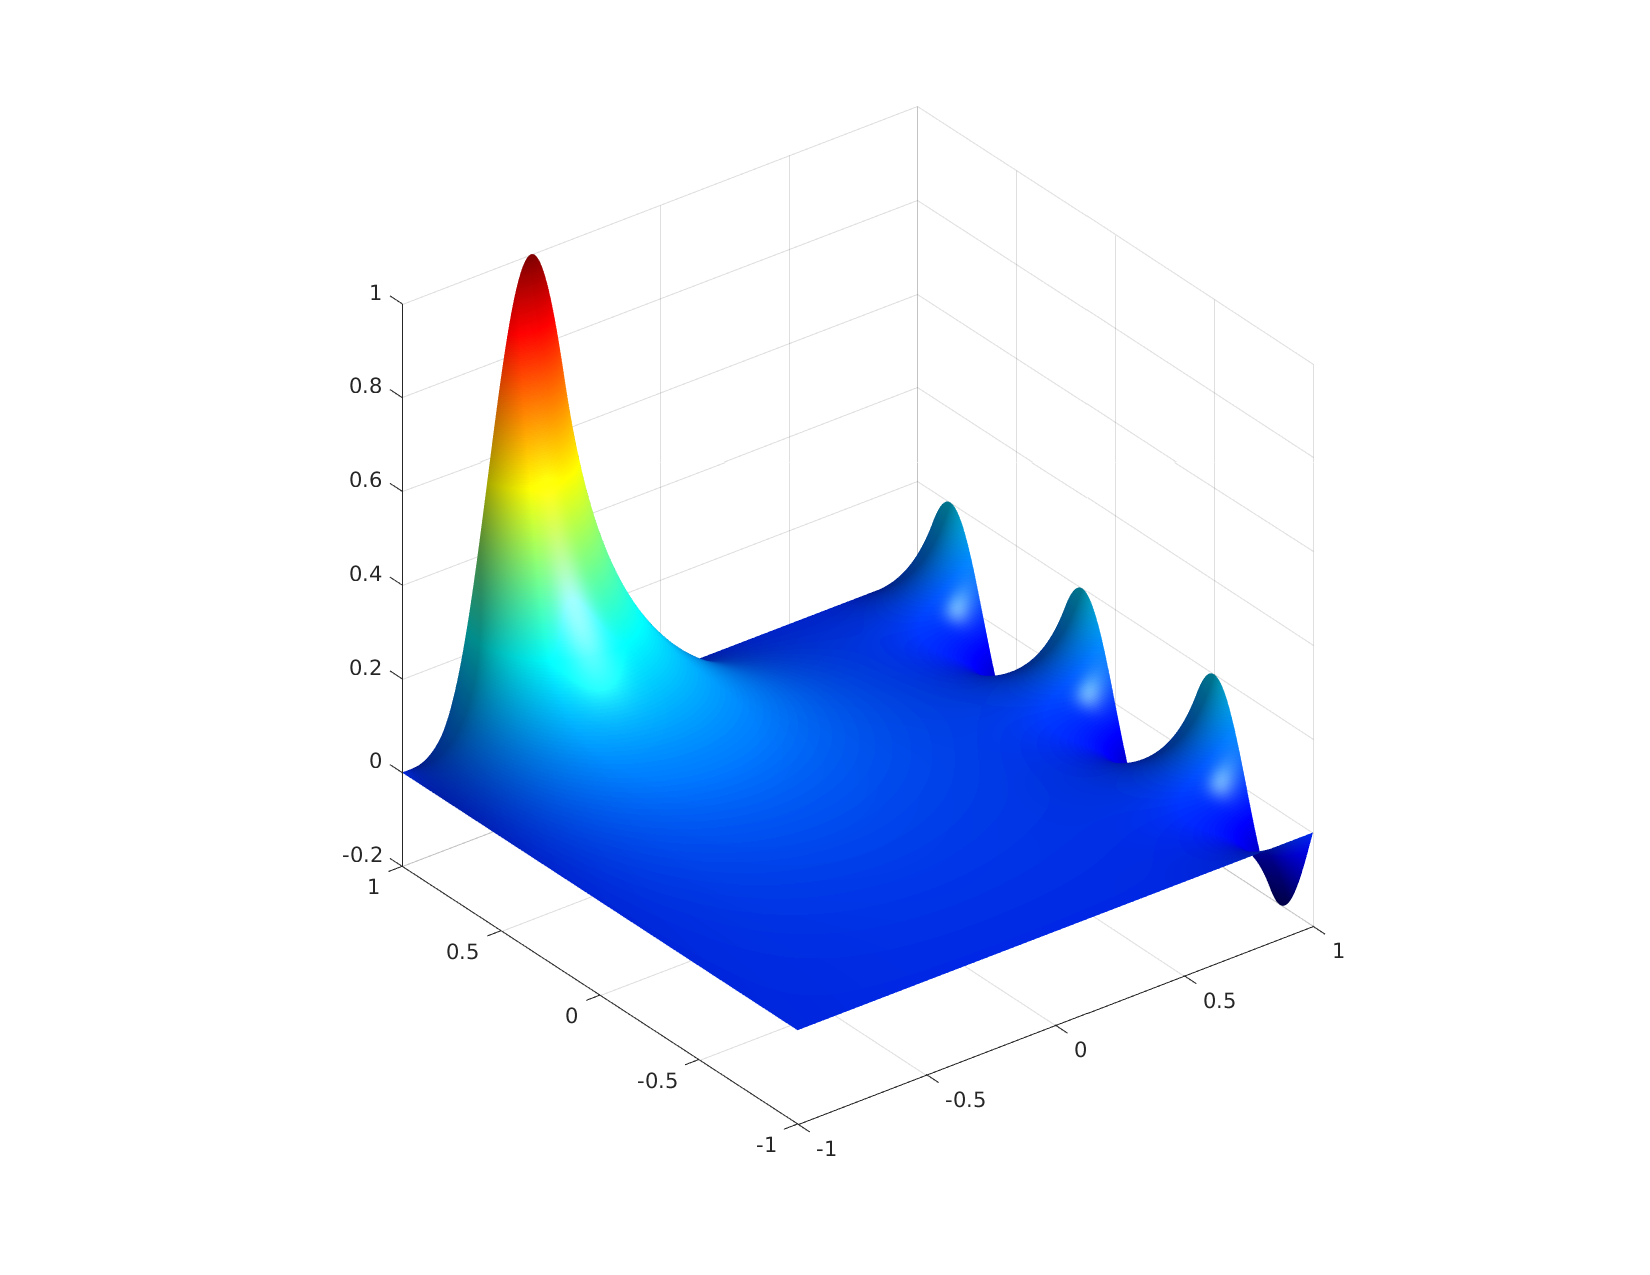
\includegraphics[width=\linewidth]{Figures/Laplace2D}
\label{fig:Laplace2D}
\end{figure}
\end{frame}

\begin{frame}{References}
\nocite{*}
\bibliographystyle{ieeetr}
\bibliography{references.bib}
\end{frame}

\end{document}